\documentclass[12pt,a4paper]{article}
\usepackage[margin=1in]{geometry}

\usepackage{polski}
\usepackage[utf8]{inputenc}

\usepackage{amsfonts}
\usepackage{amsthm}
\usepackage{enumerate}
\usepackage{graphicx}

\usepackage{indentfirst}

\author{Łukasz Bratos, Paweł Rubin}
\title{AlkoHurt - projekt bazy danych dla magazynu w hurtowni alkoholi}
\date{styczeń 2019}

\begin{document}
\maketitle

\section*{Cel projektu}

    Celem projektu jest stworzenie aplikacji bazodanowej pomagającej w zarządzaniu pojedynczym magazynem w hurtowni alkoholi. Aplikacja będzie oparta o relacyjną bazę danych z użyciem języka SQL.
    
    Aplikacja będzie udostępniać dostęp do bazy danych z trzech poziomów: administratora, kierownik i pracownika. Każdy z nich posiada dedykowane uprawnienia:
    \begin{itemize}
        \item Administrator - 
        \item Kierownik - 
        \item Pracownik - 
    \end{itemize}
    
\begin{figure}
    \centering
    
    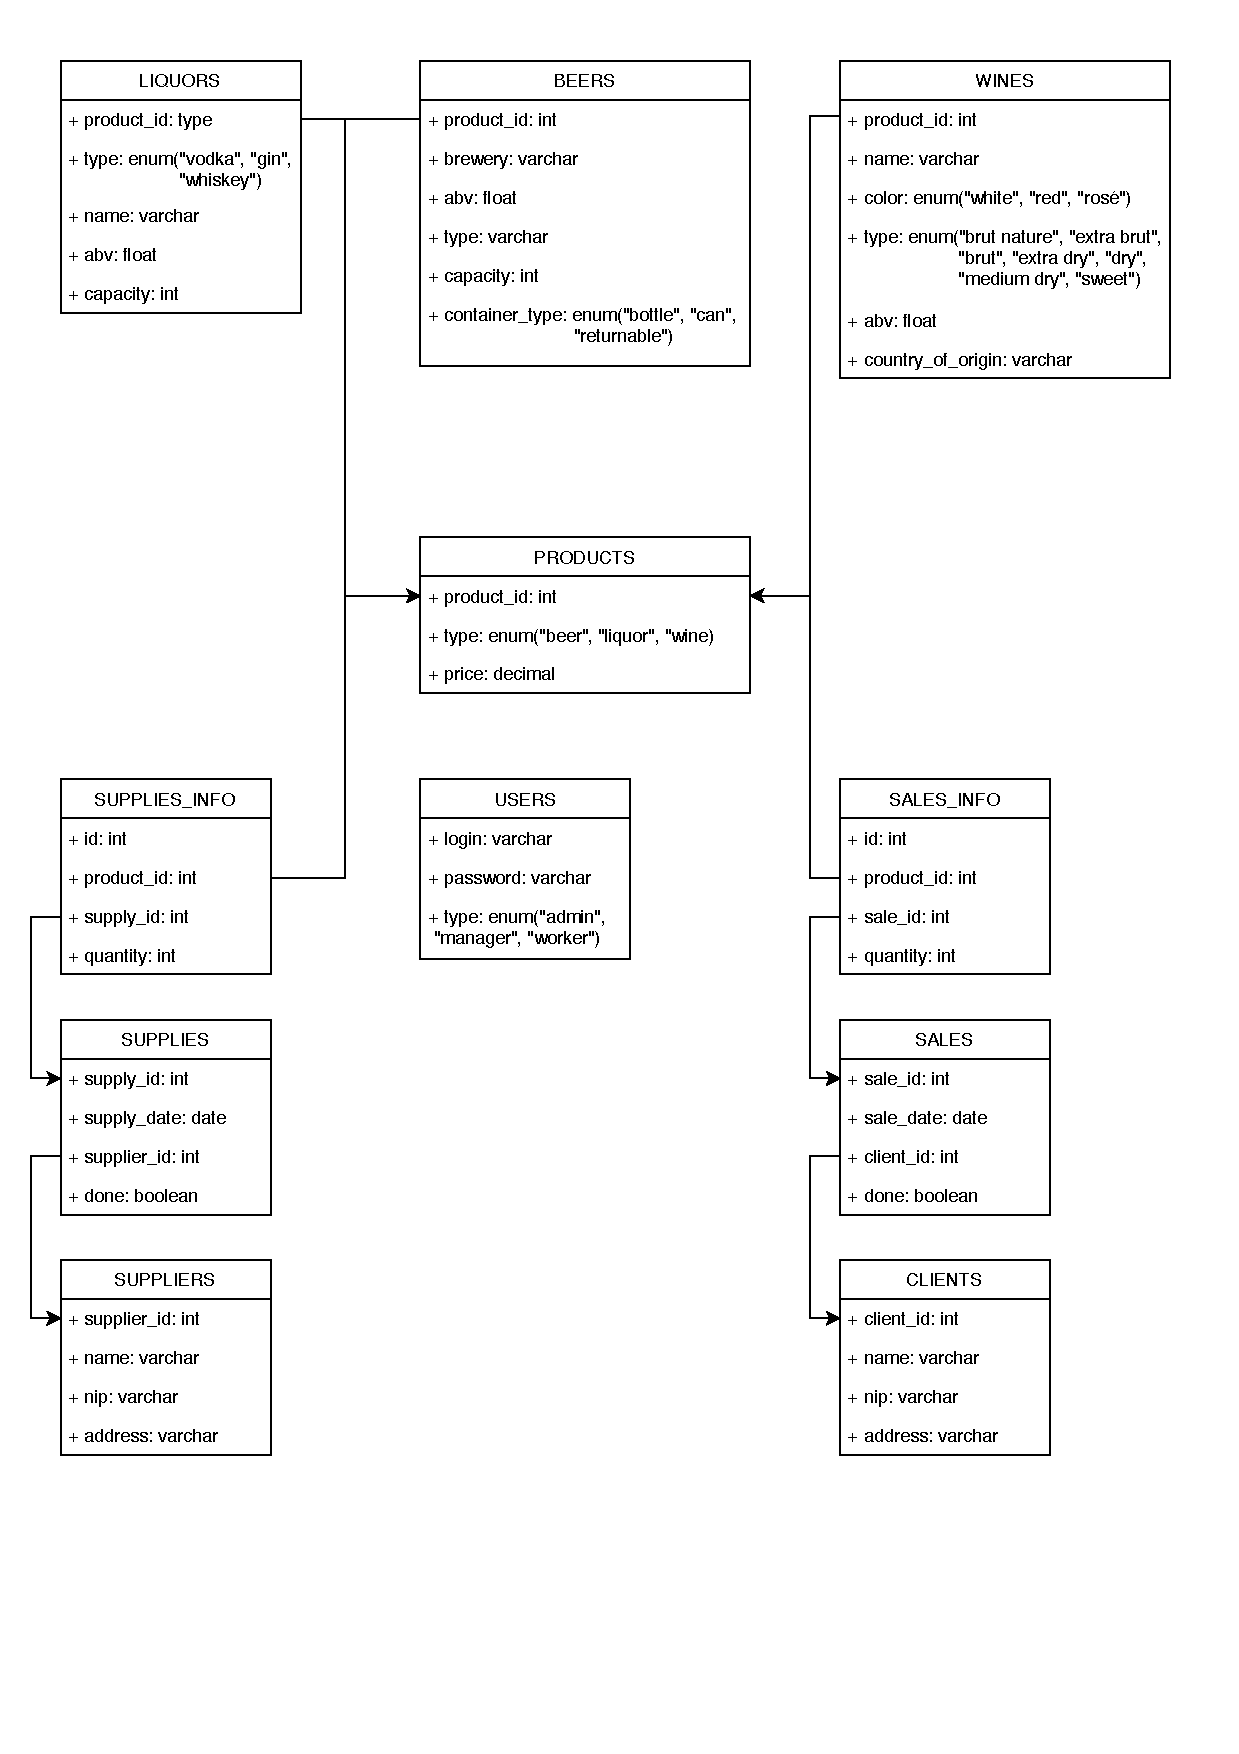
\includegraphics[width=\columnwidth]{uml}
    \caption{Diagram UML}
    \label{fig: diagram}
\end{figure}
    
    
\end{document}
